\textbf{•}\startchapter{Possibilities for Treating Experimental Data} \label{ch:6}
\section{Description}
The experimental spectra obtained from IR, Raman or SFG techniques have an amplitude scaling factor when compared to the candidate spectra generated mathematically. This means that between candidates' theoretical spectra and the experimental one, there is an unknown scaling factor. Within one particular spectroscopy technique, this scaling factor is the same for any polarization. Take IR as an example. The scaling factor for the spectrum of $x$ polarization is the same as the one for the spectrum of $z$ polarization. It is necessary to introduce this scaling factor to our LP model. \\

\section{Test Case}
\subsection{Test cases with Scaling Factor Considering Each Amino Acid Candidates from $0^{\circ}$ to $80^{\circ}$ on $\theta$ in the Mixture}
In Chapter \ref{ch:5}, the LP model constructed by Test Cases 2 to 7 in Table \ref{tab:5.1} for $\theta$ ranged from $0^{\circ}$ to $80^{\circ}$ do well in retrieving the target composition for the mixed amino acids. Therefore, based on these test cases, we investigate the LP equations can be applied directly to the real experimental data for the same $\theta$ range.\\

Therefore, the same test case settings in Table \ref{tab:5.1} are used for the following test cases. The goal is the same, that is to figure out which spectral information helps to retrieve the target composition for the mixture of six amino acids' candidates. The only difference is that, in each run of the test case set, an arbitrary scaling factor is generated for IR, Raman and SFG, respectively. Therefore, the target spectra are not only composed by the target composition of all candidates, but also need to multiple by the randomly generated scaling factors of each spectroscopy technique. \\

To start with, we limit the scaling factors to be smaller than 1. \\

After a few runs of the test case set, it is observed that the returned compositions always contains one extra variable in every test case. For Test Case 2, 4, 6 and 7, the returned composition contains the correct selected candidates. However, the percentage values of the selected candidates are different from the target composition. The ratio between the returned percentage and the target percentage are the same for all the selected candidates. Furthermore, when this ratio adds up the extra variable, it equals $1$. Randomly select one test case run as an example. Figure \ref{fig:6.2} displays the target composition, only the selected candidates are annotated with assigned percentage. Figure \ref{fig:6.2} displays the return composition of Test Case 2. The selected candidates in the return composition are correct. However, each percentage value is different from the one in the target composition. There is one extra value in Figure \ref{fig:6.2} with a value of $0.4$. \\

\begin{figure}[!ht] 
\centering
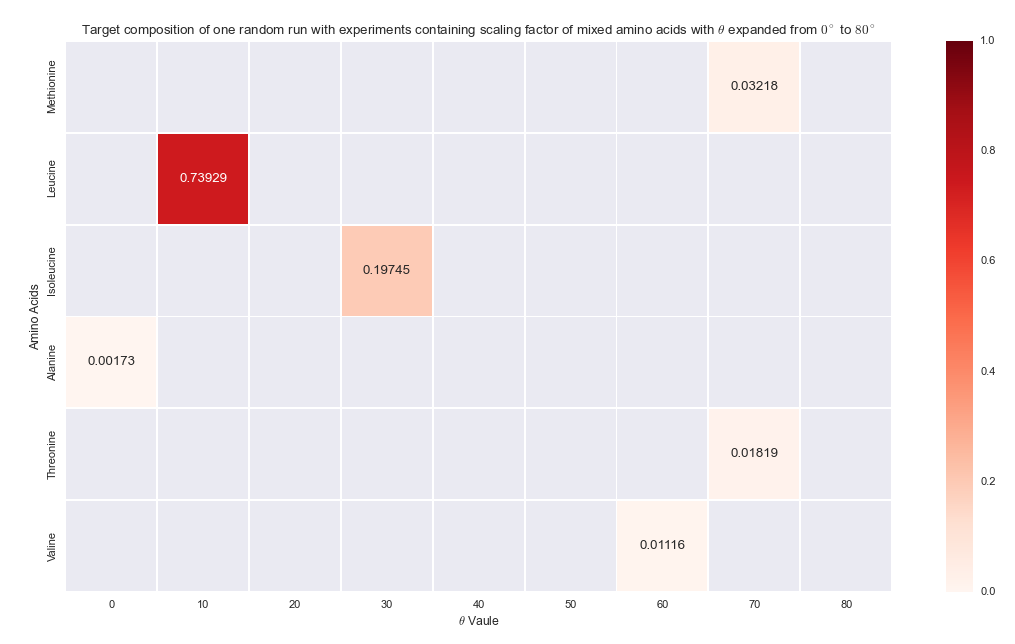
\includegraphics[scale=0.9]{Figures/chapter6_figure_one.png}
\caption{Target composition for one random run of the test case set with scaling factor for mixed amino acids, with $\theta$ expanded from $0^{\circ}$ to $80^{\circ}$. More detailed data of this target composition can be found in Appendix \ref{eqn:A.4}.} \label{fig:6.1}
\end{figure}

\begin{figure}[!ht] 
\centering
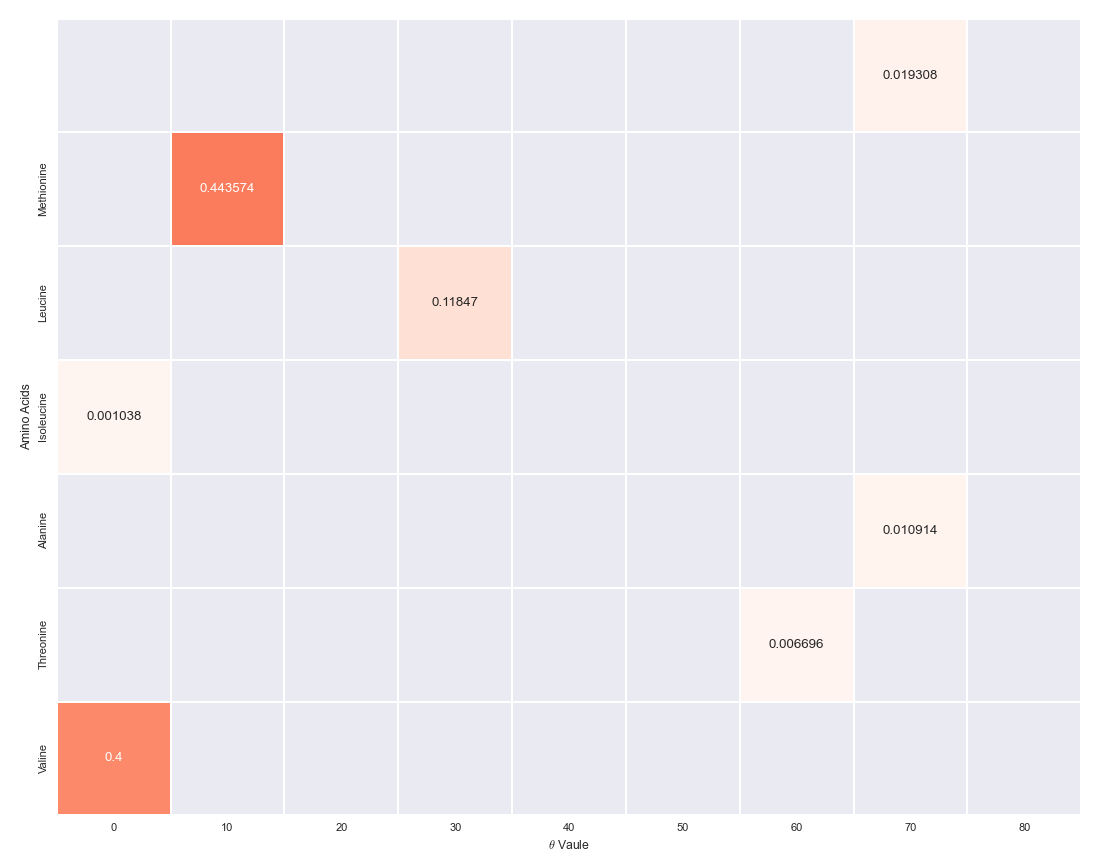
\includegraphics[scale=0.9]{Figures/chapter6_figure_two.png}
\caption{Return composition of Test Case 2 for one random run of the test case set with scaling foctor for mixed amino acids, with $\theta$ expanded from $0^{\circ}$ to $80^{\circ}$. More detailed data of this target composition can be found in Appendix \ref{eqn:A.5}.} \label{fig:6.2}
\end{figure}

\begin{figure}[!ht] 
\centering
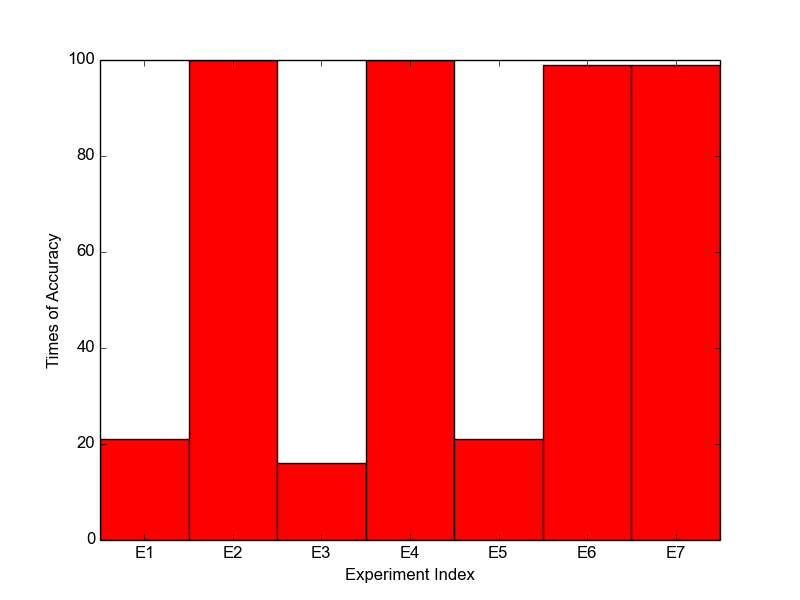
\includegraphics[scale=0.6]{Figures/chapter6_1.png}
\caption{Test case accuracy analysis for test cases using experimental spectra data that contains scaling factor that is smaller than 1 and candidates with $\theta$ from $0^{\circ}$ to $80^{\circ}$}
\label{fig:6.3}
\end{figure}

Moreover, Equation \ref{eqn:6.3} shows the ratio between the percentage of the selected candidates in the return composition and the target one is the same for all the amino acids (more precise calculated can be found in Appendix \ref{eqn:A.9}). The value of this ratio is $0.6$. When this ratio is added up with the extra variable (referred to as slack variable (SV) in LP) $0.4$, the total is $1$. As the scaling factors are pre-generated in the test case set, the value is known, which is $0.6$ for Raman spectra. In conclusion, the SV is returned by LP. Then the scaling factor (SF) equals to $1 - SV$. From the scaling factor, the ratio between the return composition and the target one is known. At the end, the target composition can be re-built from the ratio and the return composition. The re-constructed target composition matches to the original one. \\

\begin{eqnarray} \label{eqn:6.3}
\frac{0.019}{0.032} = \frac{0.44}{0.74} = \frac{0.12}{0.2} =\frac{0.001}{0.0017}  = \frac{0.011}{0.018} = \frac{0.0067}{0.011} = 0.6
\end{eqnarray}

To varify if the above observation is a general case, the test case set in Table \ref{tab:5.1} is run 100 times with randomly generated scaling factors in each run. Figure \ref{fig:6.3} indicates the test case result. Test Case 2, 4, 6 and 7 hit the above observation with almost $100\%$ frequency. This indicates that even with the scaling factor, Raman spectral information alone is sufficient to study the mixed molecules' orientation distribution at interfaces when each amino acid's candidates expanded from $0^{\circ}$ to $80^{\circ}$ on $\theta$. The target composition can be re-constructed correctly from the return slack variable and the return composition. Figure \ref{fig:6.3} also illustrates that Test Case 3 does not hit the above observation with high frequency. With the scaling factor as the addition, SFG spectral information is not sufficient to obtain the target composition. Test Case 5 indicates that even combining IR and SFG spectral information, the constructed LP model cannot help to reconstruct the target composition. This can cause by the different scaling factors of these two spectroscopy techniques. \\

\subsection{Test Cases with Scaling Factor Considering Each Amino Acid Candidates from $0^{\circ}$ to $180^{\circ}$ on $\theta$}
When each amino acid's candidates are expanded from $0^{\circ}$ to $180^{\circ}$ on $\theta$, the same test case set is applied 100 times with randomly generated scaling factors in each run. The test case result from the $100$ run illustrates that all test cases in the set meets the above observation with zero frequency. \\

However, when further analyze the return compositions of Test Case 2 and 6, there are few other observations to be noted. To facilitate the explanation, one random run is picked as an explicit example. Figure \ref{fig:6.4} is the target composition. Figure \ref{fig:6.5} and Figure \ref{fig:6.6} are the return compositions of Test Case 2 and Test Case 6. The generated scaling factor for IR, Raman and SFG are $0.863411$, $0.770505$ and $0.239947$. \\

In Figure \ref{fig:6.5}, in the return composition of Test Case 2, the slack variable equals $1-SF = 1-0.77 = 0.23$. For each amino acid, the selected candidate in the return composition may not be the exact one as shown in the target composition. However, this selected candidate is always either the correct one, or the correct one's $\theta$ complimentary. Moreover, the ratios between the percentage of each selected candidate in Figure \ref{fig:6.5} and Figure \ref{fig:6.4} are the same as shown in Equation \ref{eqn:6.2} (more precise calculated can be found in Appendix \ref{eqn:A.10}). These ratios all equal to the scaling factor of Raman. \\

In Figure \ref{fig:6.5}, for each amino acid, there are two selected candidates in the return composition. These two selected candidates are the correct one and its $\theta$ complimentary. When the percentages of these two selected candidates are added, it equals to the percentage returned for the amino acid in Figure \ref{fig:6.4}. $0.27 + 0.14 = 0.41$. Between these two selected candidates, the correct one's percentage is always bigger than its $\theta$ complement. $0.27 > 0.14$. In conclusion, Test Case 2 achieves in telling the slack variable, the scaling factor, and the ratio between the returned candidates and the target ones. However, in order to distinguish the exact candidate of each amino acid, the extra information from Test Case 6 is required. Test Case 6 tells the correct candidate from its complement on $\theta$. Together with the return information from Test Case 2 and 6, the target composition can be obtained. These observations can be applied to every run of the test case set.\\


\begin{figure}[!ht] 
\centering
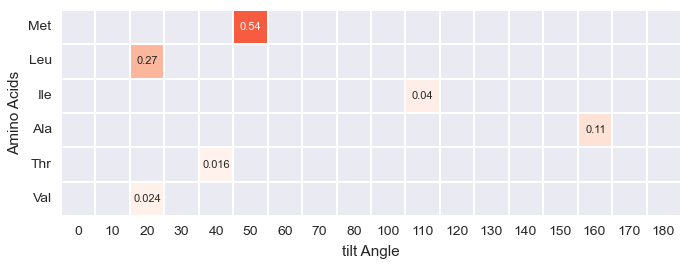
\includegraphics[scale=0.9]{Figures/chapter6_figure_five.png}
\caption{Target composition of  one random run of test cases containing scaling factor and the mixed amino acids' candidates with $\theta$ expended from $0^{\circ}$ to $180^{\circ}$. More detailed data of this target composition can be found in Appendix \ref{eqn:A.6}.} \label{fig:6.4}
\end{figure}

\begin{figure}[!ht] 
\centering
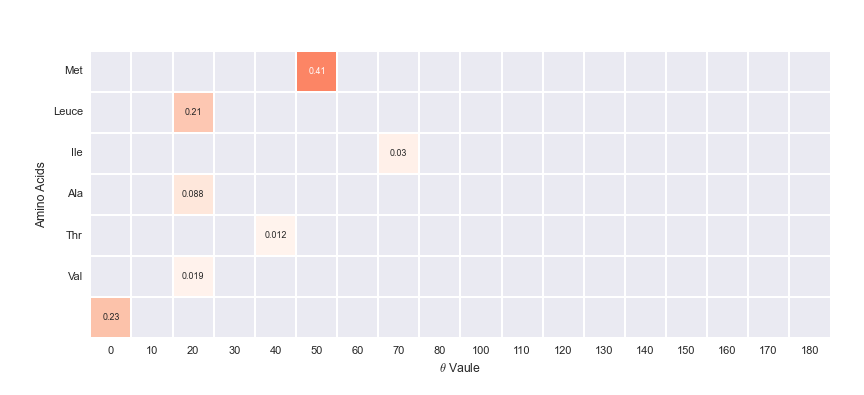
\includegraphics[scale=0.9]{Figures/chapter6_figure_three.png}
\caption{Return composition of Test Case 2 for one random run of test cases containing scaling factor and the mixed amino acids' candidates with $\theta$ expended from $0^{\circ}$ to $180^{\circ}$. More detailed data of this target composition can be found in Appendix \ref{eqn:A.7}.} \label{fig:6.5}
\end{figure}

\begin{figure}[!ht] 
\centering
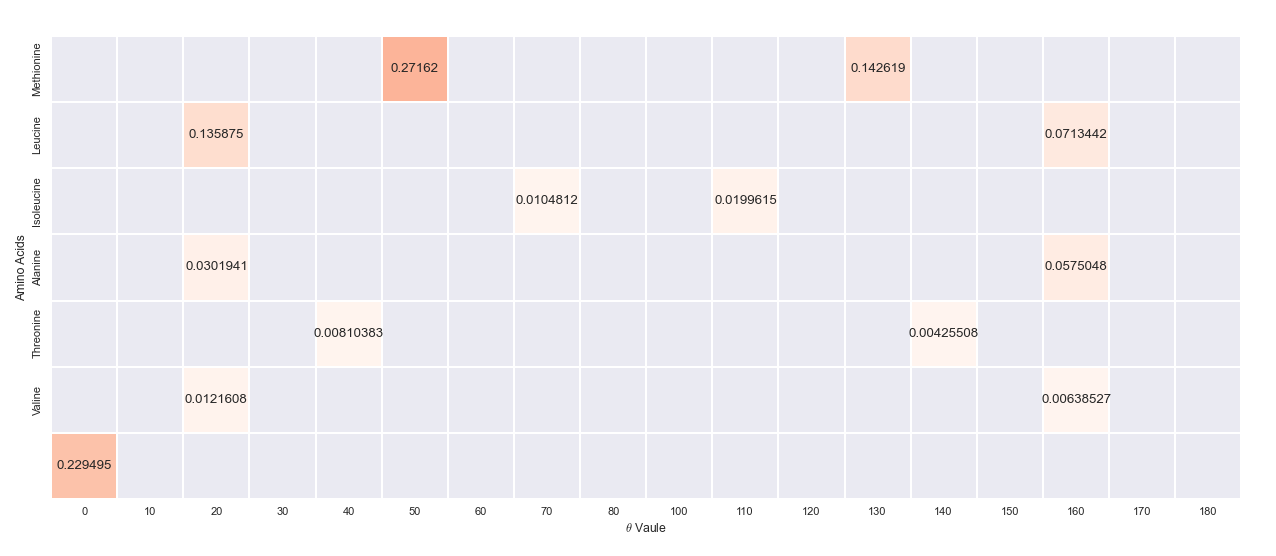
\includegraphics[scale=0.9]{Figures/chapter6_figure_four.png}
\caption{Return composition of Test Case 6 for one random run of test cases containing scaling factor and the mixed amino acids' candidates with $\theta$ expended from $0^{\circ}$ to $180^{\circ}$. More detailed data of this target composition can be found in Appendix \ref{eqn:A.8}.} \label{fig:6.6}
\end{figure}

\begin{eqnarray} 
\begin{split}
\frac{0.41}{0.54} &= \frac{0.21}{0.27} = \frac{0.03}{0.04}  =\frac{0.088}{0.11} = \frac{0.012}{0.016} = \frac{0.019}{0.024} = 0.77
\end{split}\label{eqn:6.2}
\end{eqnarray}

\section{Conclusion}

With Scaling factor introduced to different spectroscopy techniques, Raman spectral information alone is sufficient to obtain the target composition, when considering a mixture of amino acids with candidates expanded from $0^{\circ}$ to $80^{\circ}$ on $\theta$. The target composition can be re-constructed from the return SV and composition. The SF equals 1 minus SV. \\

When each amino acid's candidates are expanded from $0^{\circ}$ to $180^{\circ}$, both return compositions from Test Case 2 and 6 are needed to obtain the target composition. \\
